\documentclass[14pt, a4paper]{extarticle}
\usepackage{GOST}
\usepackage{array}
\usepackage{verbatim}
\usepackage[detect-all]{siunitx}
\usepackage{amsmath}
\usepackage{amssymb}
\usepackage[utf8]{inputenc}
\usepackage{hyperref}

\usepackage{ifthen}


\usepackage{tempora}



\makeatletter
\renewcommand\@biblabel[1]{#1.}
\makeatother

% Для листинга кода:
\usepackage{listings}
\lstset{ %
	language=c++,                 % выбор языка для подсветки (здесь это С)
	basicstyle=\small\sffamily, % размер и начертание шрифта для подсветки кода
	numbers=left,               % где поставить нумерацию строк (слева\справа)
	numberstyle=\tiny,           % размер шрифта для номеров строк
	stepnumber=1,                   % размер шага между двумя номерами строк
	numbersep=5pt,                % как далеко отстоят номера строк от подсвечиваемого кода
	showspaces=false,            % показывать или нет пробелы специальными отступами
	showstringspaces=false,      % показывать или нет пробелы в строках
	showtabs=false,             % показывать или нет табуляцию в строках
	frame=single,              % рисовать рамку вокруг кода
	tabsize=2,                 % размер табуляции по умолчанию равен 2 пробелам
	captionpos=t,              % позиция заголовка вверху [t] или внизу [b] 
	breaklines=true,           % автоматически переносить строки (да\нет)
	breakatwhitespace=false, % переносить строки только если есть пробел
	escapeinside={\#*}{*)}   % если нужно добавить комментарии в коде
}


%для графиков
\usepackage{pgfplots}
\usepackage{filecontents}
\usetikzlibrary{datavisualization}
\usetikzlibrary{datavisualization.formats.functions}

\begin{document}
	
	\begin{table}[ht]
		\centering
		\begin{tabular}{|c|p{400pt}|} 
			\hline
			\begin{tabular}[c]{@{}c@{}} 
\includegraphics[scale=1]{baum.jpg} \\\end{tabular} &
			\footnotesize\begin{tabular}[c]{@{}c@{}}\textbf{Министерство~науки~и~высшего~образования~Российской~Федерации}\\\textbf{Федеральное~государственное~бюджетное~образовательное~учреждение}\\\textbf{~высшего~образования}\\\textbf{«Московский~государственный~технический~университет}\\\textbf{имени~Н.Э.~Баумана}\\\textbf{(национальный~исследовательский~университет)»}\\\textbf{(МГТУ~им.~Н.Э.~Баумана)}\\\end{tabular}  \\
			\hline
		\end{tabular}
	\end{table}
	\noindent\rule{\textwidth}{4pt}
	\noindent\rule[14pt]{\textwidth}{1pt}
	\hfill 
	\noindent
	\makebox{ФАКУЛЬТЕТ~}%
	\makebox[\textwidth][l]{\underline{~«Информатика и системы управления»~~~~~~~~~~~~~~~~~~~~~~~~~~~~~~~~~}}%
	\\
	\noindent
	\makebox{КАФЕДРА~}%
	\makebox[\textwidth][l]{\underline{~«Программное обеспечение ЭВМ и информационные технологии»~}}%
	\\
	
	\begin{center}
		\vspace{1.5cm}
		{\bf\huge Отчёт\par}
		{\bf\Large по лабораторной работе № 4\par}
		\vspace{0.7cm}
	\end{center}
	
	
	\noindent
	\makebox{\large{\bf Название:}~~~}
	\makebox[\textwidth][l]{\large\underline{5 системных вызовов ОС UNIX/LINUX~~~~~~}}\\
	
	\noindent
	\makebox{\large{\bf Дисциплина:}~~~}
	\makebox[\textwidth][l]{\large\underline{~Операционные системы~~~~~~~~~~~~~~~~~~~~~~~~~~}}\\
	
	\vspace{1.5cm}
	\noindent
	\begin{tabular}{l c c c c c}
		Студент      & ~ИУ7-55Б~               & \hspace{2.5cm} & \hspace{2cm}                 & &  Д.В. 
		Сусликов \\\cline{2-2}\cline{4-4} \cline{6-6} 
		\hspace{3cm} & {\footnotesize(Группа)} &                & {\footnotesize(Подпись, дата)} & & {\footnotesize(И.О. Фамилия)}
	\end{tabular}
	
	\noindent
	\begin{tabular}{l c c c c}
		Преподаватель & \hspace{5cm}   & \hspace{2cm}                 & & ~~~~~~Н.Ю. Рязанова~~~~~~\\\cline{3-3} \cline{5-5} 
		\hspace{3cm}  &                & {\footnotesize(Подпись, дата)} & & {\footnotesize(И.О. Фамилия)}
	\end{tabular}
	
	\vspace{0.6cm}
	\begin{center}	
		\vfill
		\large \textit {Москва, 2020}
	\end{center}
	
	\thispagestyle {empty}
	\pagebreak
	
	% СОДЕРЖАНИЕ 
	\clearpage
	\tableofcontents
	
	
	% ВВЕДЕНИЕ
	\clearpage
	\section*{Задание 1}
	\addcontentsline{toc}{section}{Задание 1}
	Написать программу, запускающую не менее двух новых процессов системным вызовом fork(). В предке вывести собственный идентификатор (функция getpid()), идентификатор группы ( функция getpgrp()) и идентификаторы потомков. В процессе-потомке вывести собственный идентификатор, идентификатор предка (функция getppid()) и идентификатор группы. Убедиться, что при завершении процесса-предка потомок, который продолжает выполняться, получает идентификатор предка (PPID), равный 1 или идентификатор процесса-посредника.\par
	
	Программа представлена в Листинге 1.\par
	Листинг 1 - Программа 1.
	\begin{lstlisting}		
		#include <stdio.h>
		#include <stdlib.h>
		#include <unistd.h>
		
		void print_child_info(int child_num, char *status)
		{
			printf("\n%s\n\
			child:\n\
			number = %d\n\
			pid = %d\n\
			parent = %d\n\
			group = %d\n", status, child_num, getpid(),\
			 getppid(), getpgrp());
		}
		
		pid_t fork_child(int child_num)
		{
			pid_t child = fork();
			if (child == -1)
			{
				perror("fork error");
				exit(1);
			}
			else if (child == 0)
			{
				print_child_info(child_num, "S T A R T");
				sleep(3);
				print_child_info(child_num, "E N D I N G");
				exit(0);
			}
			return child;
		}
		
		int main()
		{
			pid_t child_1 = fork_child(1);
			pid_t child_2 = fork_child(2);
			pid_t child_3 = fork_child(3);
			
			printf("\nparent:\n\
			pid = %d\n\
			group = %d\n\
			child_1 = %d\n\
			child_2 = %d\n\
			child_3 = %d\n", getpid(), getpgrp(), child_1, child_2, child_3);
			
			return 0;
		}
	\end{lstlisting}
	
	\clearpage
	Результат работы программы показан на Рисунке 1.
	\begin{figure}[h]
		\centering
		
\includegraphics[scale=1]{source/1}
		\caption{Результат работы программы 1}
	\end{figure}
	
	\clearpage
	\section*{Задание 2}
	\addcontentsline{toc}{section}{Задание 2}
	Написать программу по схеме первого задания, но в процессе-предке выполнить системный вызов wait(). Убедиться, что в этом случае идентификатор процесса потомка на 1 больше идентификатора процесса-предка.\par
	
	Программа показана в Листинге 2.\par
	Листинг 2 - Программа 2.
	\begin{lstlisting}		
		#include <stdio.h>
		#include <stdlib.h>
		#include <unistd.h>
		#include <sys/types.h>
		#include <sys/wait.h>
		
		void print_child_info(int child_num, char *status)
		{
			printf("\n%s\n\
			child:\n\
			number = %d\n\
			pid = %d\n\
			parent = %d\n\
			group = %d\n", status, child_num, getpid(), getppid(), getpgrp());
		}
		
		pid_t fork_child(int child_num)
		{
			pid_t child = fork();
			if (child == -1)
			{
				perror("fork error");
				exit(1);
			}
			else if (child == 0)
			{
				print_child_info(child_num, "S T A R T");
				sleep(3);
				print_child_info(child_num, "E N D I N G");
				exit(0);
			}
			return child;
		}
		
		void wait_for_child()
		{
			int stat_val;
			pid_t child = wait(&stat_val);
			printf("Child has finished: PID = %d\n", child);
			if (WIFEXITED(stat_val))
				printf("Child = %d ended normal with code %d\n", child, WEXITSTATUS(stat_val));
			else if (WIFSIGNALED(stat_val))
				printf("Child = %d ended with a non-intercepted signal with code %d\n", child, WTERMSIG(stat_val));
			else if (WIFSTOPPED(stat_val))
				printf("Child = %d stopped with code %d\n", child, WSTOPSIG(stat_val));
		}
		
		int main()
		{
			pid_t child_1 = fork_child(1);
			pid_t child_2 = fork_child(2);
			pid_t child_3 = fork_child(3);			
			printf("\nparent:\n\
			pid = %d\n\
			group = %d\n\
			child_1 = %d\n\
			child_2 = %d\n\
			child_3 = %d\n", getpid(), getpgrp(), child_1, child_2, child_3);
			
			wait_for_child();
			wait_for_child();
			wait_for_child();
			
			return 0;
		}
	\end{lstlisting}


	\clearpage
	Результат работы программы изображен на Рисунке 2.
	\begin{figure}[h!]
		\centering
		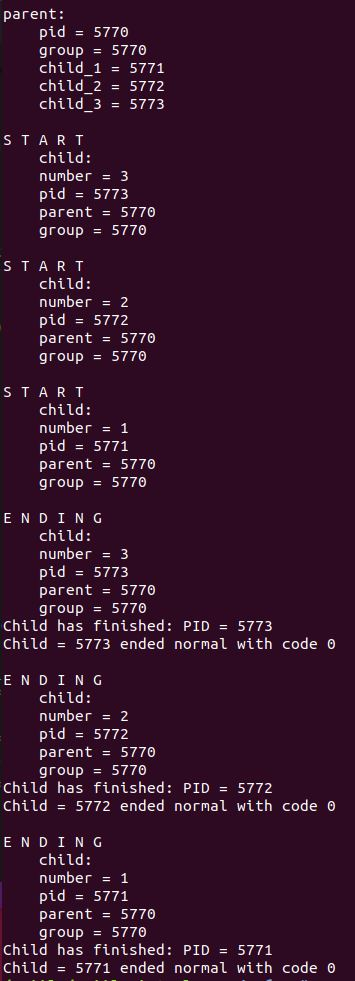
\includegraphics[scale=1]{source/2}
		\caption{Результат работы программы 2}
	\end{figure}

	\clearpage
	\section*{Задание 3}
	\addcontentsline{toc}{section}{Задание 3} 
	Написать программу, в которой процесс-потомок вызывает системный вызов exec(), а процесс-предок ждет завершения процесса-потомка. Следует создать не менее двух потомков.\par
	
	Программа представлена в Листинге 3.\par
	Листинг 3 - Программа 3.
	\begin{lstlisting}		
		#include <stdio.h>
		#include <stdlib.h>
		#include <unistd.h>
		#include <sys/types.h>
		#include <sys/wait.h>
		
		void print_child_info(int child_num)
		{
			printf("\nchild:\n\
			number = %d\n\
			pid = %d\n\
			parent = %d\n\
			group = %d\n", child_num, getpid(), getppid(), getpgrp());
		}
		
		pid_t fork_child(int child_num, char *path, char *arg0)
		{
			pid_t child = fork();
			if (child == -1)
			{
				perror("fork error");
				exit(1);
			}
			else if (child == 0)
			{
				print_child_info(child_num);
				if (execl(path, arg0, NULL) == -1)
				{
					perror("exec error");
					exit(1);
				}
				
			}
			return child;
		}
		
		void wait_for_child()
		{
			int stat_val;
			pid_t child = wait(&stat_val);
			printf("Child has finished: PID = %d\n", child);
			if (WIFEXITED(stat_val))
				printf("Child %d ended normal with code %d\n", child, WEXITSTATUS(stat_val));
			else if (WIFSIGNALED(stat_val))
				printf("Child %d ended with a non-intercepted signal with code %d\n", child, WTERMSIG(stat_val));
			else if (WIFSTOPPED(stat_val))
				printf("Child %d stopped with code %d\n", child, WSTOPSIG(stat_val));
		}
		
		int main()
		{
			pid_t child_1 = fork_child(1, "/bin/ls", "ls");
			pid_t child_2 = fork_child(2, "/bin/ps", "ps");
			
			printf("\nparent:\n\
			pid = %d\n\
			group = %d\n\
			child_1 = %d\n\
			child_2 = %d\n", getpid(), getpgrp(), child_1, child_2);
			
			wait_for_child();
			wait_for_child();
			
			return 0;
		}
	\end{lstlisting}

	Результат работы программы показан на Рисунке 3.
	\begin{figure}[h!]
		\centering
		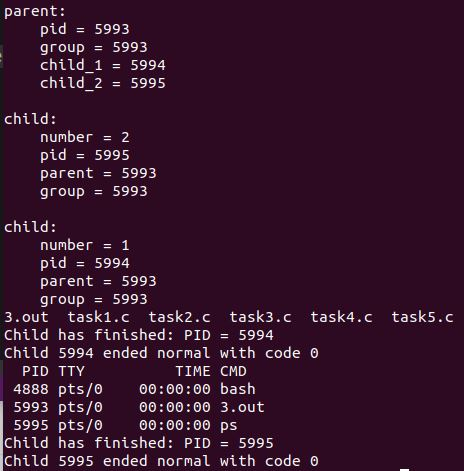
\includegraphics[scale=1]{source/3}
		\caption{Результат работы программы 3}
	\end{figure}


	 \clearpage
	 \section*{Задание 4}
	 \addcontentsline{toc}{section}{Задание 4}
	 Написать программу, в которой предок и потомок обмениваются сообщением через программный канал.\par
	 Программа показана в Листинге 4.\par
	 Листинг 4 - Программа 4.
	 \begin{lstlisting}		
	 	#include <stdio.h>
	 	#include <stdlib.h>
	 	#include <unistd.h>
	 	#include <sys/types.h>
	 	#include <sys/wait.h>
	 	
	 	pid_t fork_child(int child_num, int *fd)
	 	{
	 		pid_t child = fork();
	 		if (child == -1)
	 		{
	 			perror("fork error");
	 			exit(1);
	 		}
	 		else if (child == 0)
	 		{
	 			int pid_int = getpid();
	 			void* pid = &pid_int;
	 			close(fd[0]);
	 			write(fd[1], pid, sizeof(pid));
	 			exit(0);
	 		}
	 		return child;
	 	}
	 	
	 	void wait_for_child(int *fd)
	 	{
	 		int stat_val;
	 		void* pid = malloc(sizeof(void*));
	 		
	 		close(fd[1]);
	 		read(fd[0], pid, sizeof(pid));
	 		
	 		pid_t child = wait(&stat_val);
	 		printf("Child %d send %d\n", child, *(int*)pid);
	 		if (WIFEXITED(stat_val))
	 		printf("Child %d completed normally with code %d\n", child, WEXITSTATUS(stat_val));
	 		else if (WIFSIGNALED(stat_val))
	 		printf("Child %d ended with a non-intercepted signal with code %d\n", child, WTERMSIG(stat_val));
	 		else if (WIFSTOPPED(stat_val))
	 		printf("Child %d stopped with code %d\n", child, WSTOPSIG(stat_val));
	 		
	 		free(pid);
	 	}
	 	
	 	int main()
	 	{
	 		int fd[2];
	 		if (pipe(fd) == -1)
	 		{
	 			perror("pipe error");
	 			exit(1);
	 		}
	 		
	 		pid_t child_1 = fork_child(1, fd);
	 		pid_t child_2 = fork_child(2, fd);
	 		
	 		printf("\nparent:\n\
	 		pid = %d\n\
	 		group = %d\n\
	 		child_1 = %d\n\
	 		child_2 = %d\n", getpid(), getpgrp(), child_1, child_2);
	 		
	 		wait_for_child(fd);
	 		wait_for_child(fd);
	 		
	 		return 0;
	 	}
	 \end{lstlisting}
	 
	 Результат работы программы изображен на Рисунке 4.
	 \begin{figure}[h!]
	 	\centering
	 	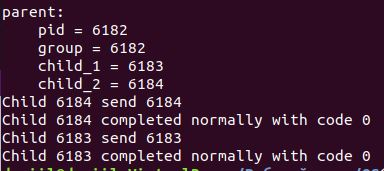
\includegraphics[scale=1]{source/4}
	 	\caption{Результат работы программы 4}
	 \end{figure}
 
 	\clearpage
 	\section*{Задание 5}
 	\addcontentsline{toc}{section}{Задание 5}
 	В программу с программным каналом включить собственный обработчик сигнала. Использовать сигнал для изменения хода выполнения программы.\par
 	Программа представлена в Листинге 5.\par
 	Листинг 5 - Программа 5.
 	\begin{lstlisting}		
	 	#include <stdio.h>
	 	#include <stdlib.h>
	 	#include <unistd.h>
	 	#include <sys/types.h>
	 	#include <sys/wait.h>
	 	#include <string.h>
	 	
	 	int flag = 0;
	 	
	 	void catch_signal(int sig_numb)
	 	{
	 		printf("\nCatch signal Cntrl + Z\n");
	 		flag = 1;
	 	}
	 	
	 	void waiting_for_signal()
	 	{
	 		printf("Press Ctrl + Z to continue\n");
	 		signal(SIGTSTP, catch_signal);
	 		sleep(3);
	 	}
	 	
	 	pid_t fork_child(int child_num, int *fd)
	 	{
	 		pid_t child = fork();
	 		if (child == -1)
	 		{
	 			perror("fork error");
	 			exit(1);
	 		}
	 		else if (child == 0)
	 		{
	 			if (flag)
	 			{
	 				int pid_int = getpid();
	 				void* pid = &pid_int;
	 				close(fd[0]);
	 				write(fd[1], pid, sizeof(pid));
	 			}
	 			exit(0);
	 		}
	 		return child;
	 	}
	 	
	 	void wait_for_child(int *fd)
	 	{
	 		int stat_val;
	 		void *pid = (void*)malloc(sizeof(void*));
	 		pid_t child = wait(&stat_val);
	 		if (flag)
	 		{
	 			close(fd[1]);
	 			read(fd[0], pid, sizeof(pid));
	 			printf("Child %d send %d\n", child, *(int*)pid);
	 		}
	 		else
	 		printf("Child %d send NONE\n", child);
	 		
	 		if (WIFEXITED(stat_val))
	 		printf("Child %d completed normally with code %d\n", child, WEXITSTATUS(stat_val));
	 		else if (WIFSIGNALED(stat_val))
	 		printf("Child %d ended with a non-intercepted signal with code %d\n", child, WTERMSIG(stat_val));
	 		else if (WIFSTOPPED(stat_val))
	 		printf("Child %d stopped with code %d\n", child, WSTOPSIG(stat_val));
	 		
	 		free(pid);
	 	}
	 	
	 	int main()
	 	{
	 		int fd[2];
	 		
	 		if (pipe(fd) == -1)
	 		{
	 			perror("pipe error");
	 			exit(1);
	 		}
	 		
	 		waiting_for_signal();
	 		
	 		pid_t child_1 = fork_child(1, fd);
	 		pid_t child_2 = fork_child(2, fd);
	 		
	 		printf("\nparent:\n\
	 		pid = %d\n\
	 		group = %d\n\
	 		child_1 = %d\n\
	 		child_2 = %d\n", getpid(), getpgrp(), child_1, child_2);
	 		
	 		wait_for_child(fd);
	 		wait_for_child(fd);
	 		
	 		return 0;
	 	}
 	\end{lstlisting}
 	
 	Результат работы программы при перехвате сигнала показан на Рисунке 5.
 	\begin{figure}[h!]
 		\centering
 		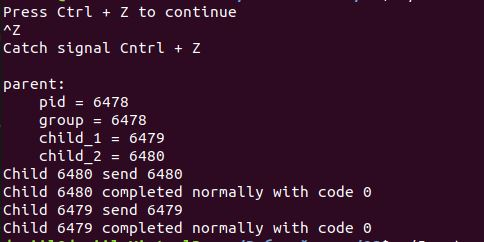
\includegraphics[scale=1]{source/5}
 		\caption{Результат работы программы 5 при перехвате сигнала}
 	\end{figure}
 	
	Результат работы программы при отсутствии сигнала изображен на Рисунке 6.
	\begin{figure}[h!]
		\centering
		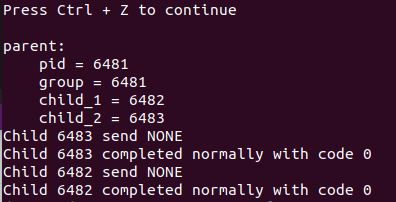
\includegraphics[scale=1]{source/6}
		\caption{Результат работы программы 6 при отсутствии сигнала}
	\end{figure}
\end{document}